\newpage
\appendix
\section{Appendix}

\subsection{Proof of consistency theorem}
\label{appendix:theorem_proof}

Proof of the theorem in \ref{sec:theorem}:


\begin{theorem}[B2B consistency - general case]

     Consider the B2B model from equation \ref{eq:model} $$Y = (XE + N)F$$ with $N$ centred and full rank noise.

     If $F$ and $X$ are full-rank on $Img(E)$, then, the solution of B2B, $\hat H$ minimizes

     $$\min_H  \left \| X - XH\right\| ^2  + \left \| NH\right \| ^2$$ and satisfies

     $$E\hat H = \hat H$$
\end{theorem}
\begin{proof}

 Let $\hat G$ and $\hat H$ be the solutions of the first and second regressions of B2B.

 Since $\hat G$ is the least square estimator of $X$ from $Y$
 \begin{align*}
    \hat G = \arg \min_G \mathbb{E}[\left \| YG - X \right \|^2]
\end{align*}
Replacing $Y$ by its model definition $Y = (XE+N)F$, we have
 \begin{align*}
    \hat G &=   \arg \min_G \mathbb{E}[\left \| X - (XE + N)FG \right\|^2] =\arg \min_G \mathbb{E}[\left \| X - XEFG + NFG \right\|^2]
  \end{align*}
  Since $N$ is centered and independent of $X$, we have
  \begin{align}
    	  \hat G &=  \arg \min_G \left \| X - XEFG\right\| ^2  + \left \| NFG\right \| ^2
     \label{eq:Gdoublenorm}
\end{align}

Samely, for $\hat H$, we have
\begin{align*}
    \hat H = \arg \min_H \mathbb{E}[\| XH - Y \hat{G} \|^2] &=\arg  \min_H \mathbb{E}[\| XH - (XE + N)F \hat G \|^2] \\
    &=\arg \min_H \mathbb{E}[\| X(H - EF \hat G) \| ^2] + \mathbb{E}[\| NF\hat G \| ^2]\\
    &= \arg \min_H \mathbb{E}[\| X(H - EF \hat G) \| ^2]
 \end{align*}
 a positive quantity which reaches a minimum (zero) for
 \begin{align}
    \hat H = EF \hat G
    \label{eq:Hdoublenom}
\end{align}

Let us now prove that $EF\hat G = F\hat G$.

Let $F^\dagger$ be the pseudo inverse of $F$, and $Z=F^\dagger EF\hat G$, we have $FZ = FF^\dagger EF \hat G$

Since $F$ is full rank on $Img(E)$, we have $FF^\dagger E =E$, and $FZ = EF\hat G$

As $E$ is a binary diagonal matrix, it is an orthogonal projection and therefore a contraction, thus
 $$ \| NEF\hat G\|^2 \leq \| NF\hat G \|^2$$ and
 $$\left \| X - XEFZ\right \| ^2  + \left \| NFZ\right \| ^2 = \| X - XEF\hat G \| ^2  + \| NEF\hat G \| ^2 \leq \| X - XEF\hat G \| ^2  + \| NF\hat G \| ^2$$

But since $\hat G =  \arg \min_G \left \| X - XEFG\right\| ^2  + \left \| NFG\right \| ^2$, we also have
$$\left \| X - XEF\hat G\right\| ^2  + \left \| NF\hat G\right \| ^2 \leq \left \| X - XEFZ\right \| ^2  + \left \| NFZ\right \| ^2$$

Summarizing the above,
$$\left \| X - XEF\hat G\right\| ^2  + \left \| NF\hat G\right \| ^2 \leq \| X - XEF\hat G \| ^2  + \| NEF\hat G \| ^2 \leq \| X - XEF\hat G \| ^2  + \| NF\hat G \| ^2$$
$$\left \| X - XEF\hat G\right\| ^2  + \left \| NF\hat G\right \| ^2 = \| X - XEF\hat G \| ^2  + \| NEF\hat G \| ^2$$
$$\left \| NF\hat G\right \| ^2 =  \| NEF\hat G \| ^2$$

$N$ being full rank, this yields $EF\hat G = F\Hat G$.

Replacing into $\eqref{eq:Gdoublenorm}$, and setting $H = EFG$, we have
\begin{align*}
	\hat G &=  \arg \min_G  \left \| X - XEFG\right \| ^2  + \left \| NFG\right \| ^2 \\
	&=   \arg \min_G \left \| X - XEFG\right \| ^2  + \left \| NEFG\right \| ^2 \\
	\hat H &=  \arg \min_H \left \| X - XH\right \| ^2  + \left \| NH\right \| ^2
	\label{eq:4}
\end{align*}

Finally, $E\hat H = E EF\hat G = EF\hat G = \hat H$, since $E$, a binary diagonal matrix, is involutive. This completes the proof.
\end{proof}



\newpage
\subsection{Modeling measurement noise}

Equation \ref{eq:model} does not explicitly contain a measurement noise term. Yet, in moast experimental cases, the problem is best described as:
\begin{equation}
  Y = (XE+N)F+M
  \label{eq:model_noisy_measure}
\end{equation}
  with $M\in \mathbb{R}^{n \times d_y}$.

This equation is actually equivalent to Equation \ref{eq:model} given our hypotheses. Indeed, we can rewrite $M = MF^{-1}F$ over $Img(F)$, which leads to:
$$Y = (XE+N)F+M = (XE+N+MF^{-1})F = (XE+N')F$$

Consequently, assuming that $F$ is full rank on $Img(XE)$, B2B yields the same solutions to equations \ref{eq:model} and \ref{model_noisy_measure}.


\subsection{Feature importance}
\label{appendix:feature_importance}

For B2B, feature importance is assessed as follows:

\begin{algorithm}[H]
    %\SetAlgoLined
    \KwIn{$X_{train} \in \mathbb{R}^{n \times d_x}$, $X_{test} \in
\mathbb{R}^{n' \times d_x}$, $Y_{train} \in \mathbb{R}^{n\times d_y}$, $Y_{test}
\in \mathbb{R}^{n'\times d_y}$, } \KwOut{estimate of prediction improvement
$\Delta{R} \in \mathbb{D}^{d_x}$.} $H, G = \text{B2B}(X_{train}, Y_{train})$\;
$R_{full} = \text{corr}(X_{test} H, Y_{test} G)$\;

    \For{$i = 1, \ldots, d_x$}{ $K = Id$\; $K[i] \leftarrow 0$\;
    $R_{k} =
\text{corr}(X_{test} K H, Y_{test} G_i)$\; $\Delta R_i = R_{full} - R_{k}$\; }
\Return{$\Delta R$} \caption{B2B feature importance.} \label{algorithm:b2b_fi}
\end{algorithm}

For the Forward Model, the feature importance is assessed as follows:

\begin{algorithm}[H]
    %\SetAlgoLined
    \KwIn{$X_{train} \in \mathbb{R}^{n \times d_x}$, $X_{test} \in
\mathbb{R}^{n' \times d_x}$, $Y_{train} \in \mathbb{R}^{n\times d_y}$, $Y_{test}
\in \mathbb{R}^{n'\times d_y}$, } \KwOut{estimate of prediction improvement
$\Delta{R} \in \mathbb{D}^{d_x, d_y}$.}

$H = \text{LinearRegression}(X_{train}, Y_{train})\;
R_{full} = \text{corr}(X_{test} K, Y_{test})$\;

    \For{$i = 1, \ldots, d_x$}{ $K = Id$\; $K[i] \leftarrow 0$\; $R_{k} = \text{corr}(X_{test}
K H, Y_{test})$\; $\Delta R_i = R_{full} - R_{k}$\; } \Return{$\Delta R$}
\caption{Forward feature importance.} \label{algorithm:fwd_fi} \end{algorithm}

% \iffalse
% \begin{enumerate}
%   \item Fit $H$ given $X_{train}$ and $Y_{train}$
%   \item For each feature $i$:
%   \begin{itemize}
%     \item Define $K$, and identity matrix whose row $i$ has been zeroed-out
%     \item Fit $H^i_k$ given $X_{train} K$ and $Y_{train}$
%   \end{itemize}
%   \end{enumerate}
% \fi

For the CCA and PLS models, the feature importance is assessed as follows:

\begin{algorithm}[H]
    %\SetAlgoLined
    \KwIn{$X_{train} \in \mathbb{R}^{n \times d_x}$, $X_{test} \in
\mathbb{R}^{n' \times d_x}$, $Y_{train} \in \mathbb{R}^{n\times d_y}$, $Y_{test}
\in \mathbb{R}^{n'\times d_y}$, } \KwOut{estimate of prediction improvement
$\Delta{R} \in \mathbb{D}^{d_x, d_z}$.} $H, G = \text{CCA}(X_{train},
Y_{train})$\; $R_{full} = \text{corr}(X_{test} H, Y_{test} G)$\;

    \For{$i = 1, \ldots, d_x$}{ $K = Id$\; $K[i] \leftarrow 0$\; $R_{k} = \text{corr}(X_{test} K H,
Y_{test} G)$\; $\Delta R_i = R_{full} - R_{k}$\; } \Return{$\Delta R$}
\caption{CCA and PLS feature importance.} \label{algorithm:cdp_fi}
\end{algorithm}

For the Backward Model, feature importance cannot be assessed because there is no prediction.

\subsection{Binarizing $\hat{H}$ - the Sonquist-Morgan criterion}

Back to back regression provides us with $Diag(\hat{H})$, a vector of real numbers that estimate the causal influence of features in $X$. In order to derive the true causal influence matrix $E$ , a binary matrix, we need to binarize  $\hat{H}$, i.e. test each feature for equality with zero. In regression analysis, the traditional approach to this problem employs a $t$-test to check whether the regression coefficients differ from zero \citep{student1908probable}. This test will not succeed here: $\hat{H}$ is obtained from a double regression with regularization, and will not follow the t-distribution.

Instead, we treat the binarization of $\hat{H}$ as a clustering problem: separate the elements in the diagonal into a group of ``small values'', and a group of ``large values''. More specifically, we propose to maximize the ratio of inter-group variance and to minimize the intra-group variance, over all possible splits of the diagonal into $p$ largest values and $d_x-p$ smallest values.
%
Letting $m_0$ and $m_1$ be the average values of the two clusters, $p$ and $d_x-p$ their size, and $v$ the total variance of the sample, we select the split maximizing the Sonquist-Morgan \citep{sonquist_morgan} \citep{kass75} criterion $\frac{p(d_x-p)}{d_x} \frac{(m_1 - m_0)^2}{v}$.
%
To binarize $\hat{H}$, set to one all the $p$ diagonal entries belonging to the ``large values'' group in the decided split, and setting to zero the rest of the $d_x-p$ diagonal entries.


\section{Additional Figures}


% \begin{figure}[t!]
%   \centering
%   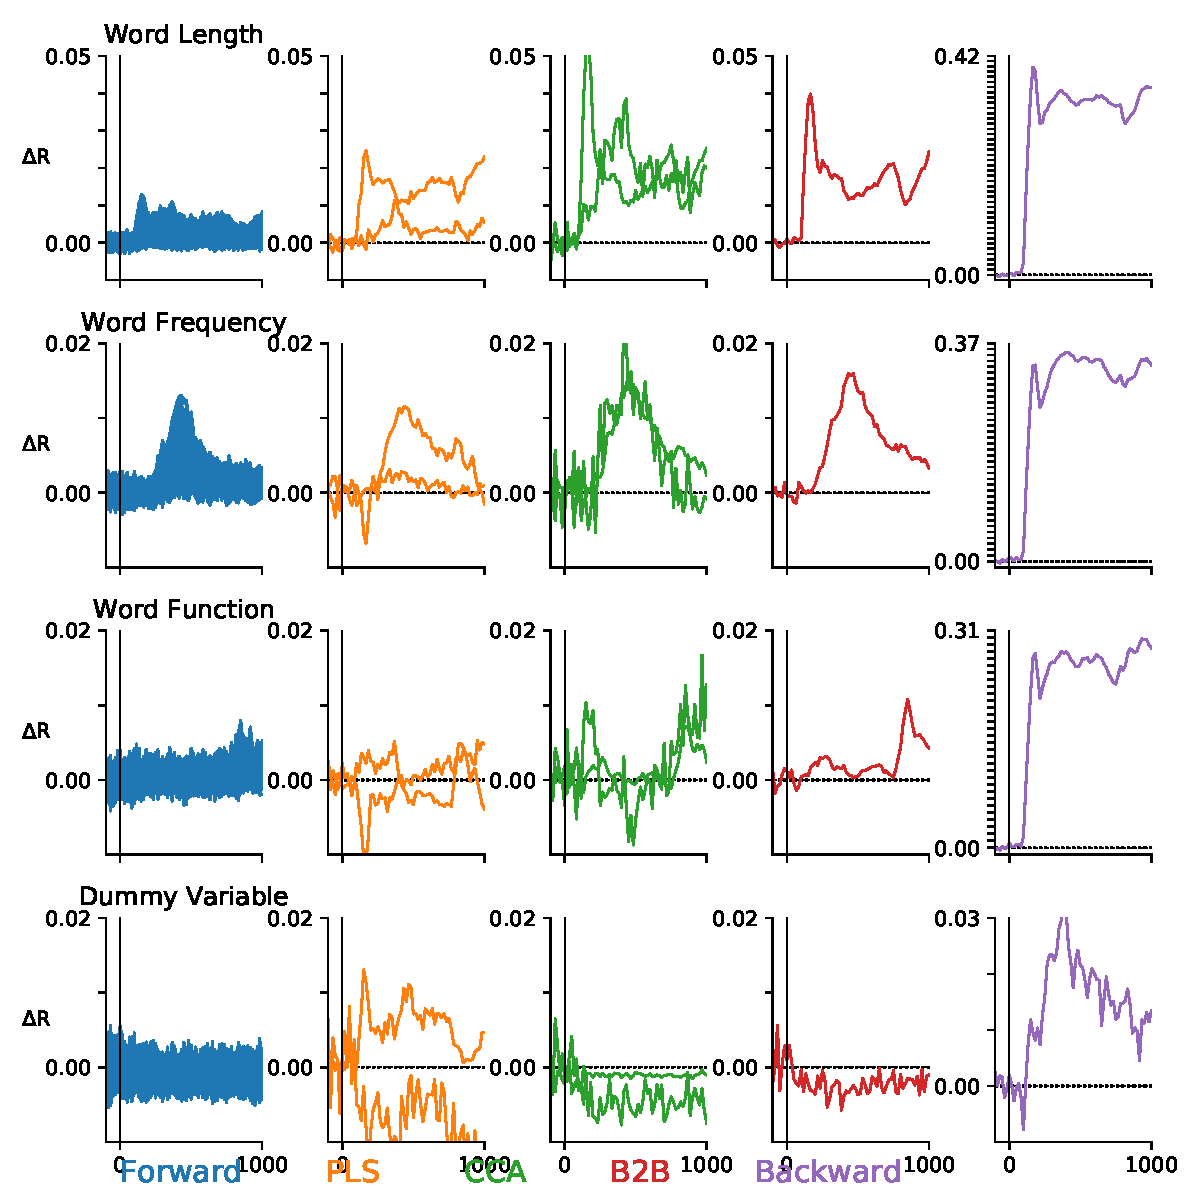
\includegraphics[width=\textwidth, trim=0cm 0cm 0cm 0cm, clip=True]{figures/meg_supp.pdf}
%   \caption{Average $\Delta R$ for each $Y$ dimension (Forward model), canonical components (PLS and CCA) or feature (B2B) across subjects. Formally, Backward model cannot have a $\Delta R$ because it never unmixes the multiple $X$ features. In such cases, we thus simply report the decoding score.}
%   \label{fig:meg_supp}
% \end{figure}


\begin{figure}
  \centering
  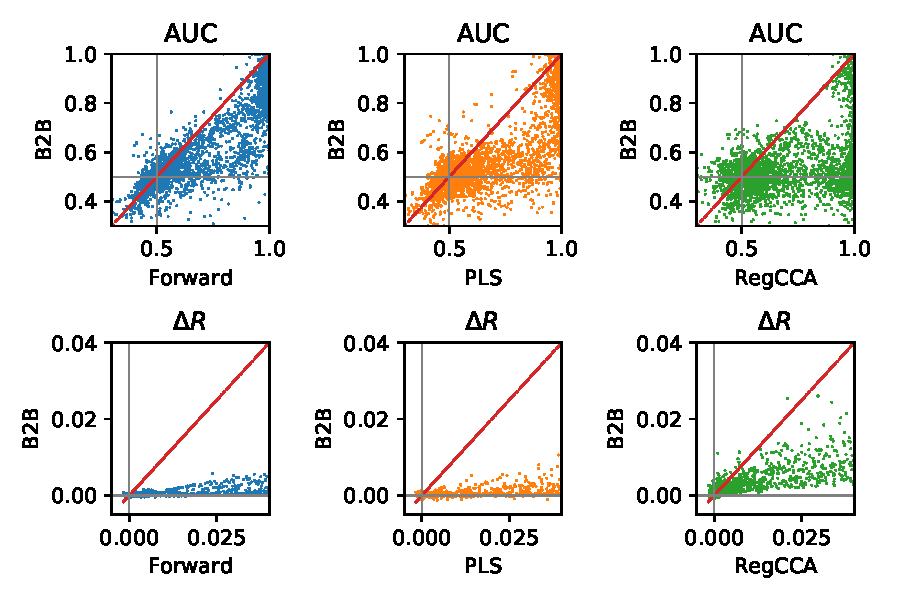
\includegraphics[width=\linewidth]{figures/delta_auc.pdf}
  \caption{Synthetic experiments. Distribution (over conditions) of AUC (top) and Feature Importance $\Delta R$ (bottom) metrics between our method (y-axis) and the baselines (x-axis). Each dot is a distinct synthetic experiment. Dots below the diagonal indicates that B2B outperform the tested model. \label{fig:auc_plots}}
\end{figure}

\begin{figure}
  \centering
  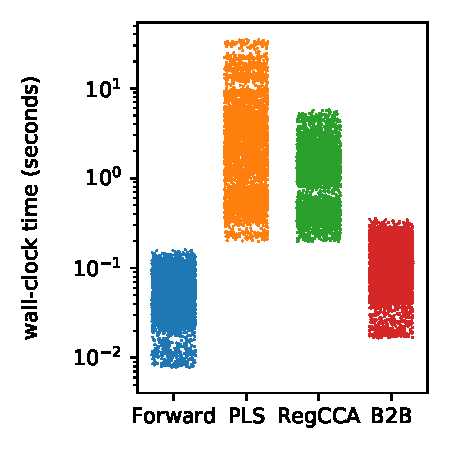
\includegraphics[width=0.7\linewidth]{figures/duration}
  \caption{Wall-clock run-time for our method B2B and for the baselines. Each dot is a distinct synthetic experiment. B2B runs much faster than cross-decomposition baselines. \label{fig:duration}}
\end{figure}


\subsection{Robustness to increasing number of factors}

To test whether each of the methods robustly scales to an increasingly large number of potential causes $X$, we enhanced the four ad-hoc features (word length, word frequency, word function, dummy variable) with another ten features. These additional features corresponds to the first dimensions of word embedding as provided by Spacy \citep{spacy2}. The results shown in Figure \ref{fig:embbedings}, show that the feature importance of ad-hoc features as derived by B2B remain unchanged (and are actually improved).

\begin{figure}
  \centering
  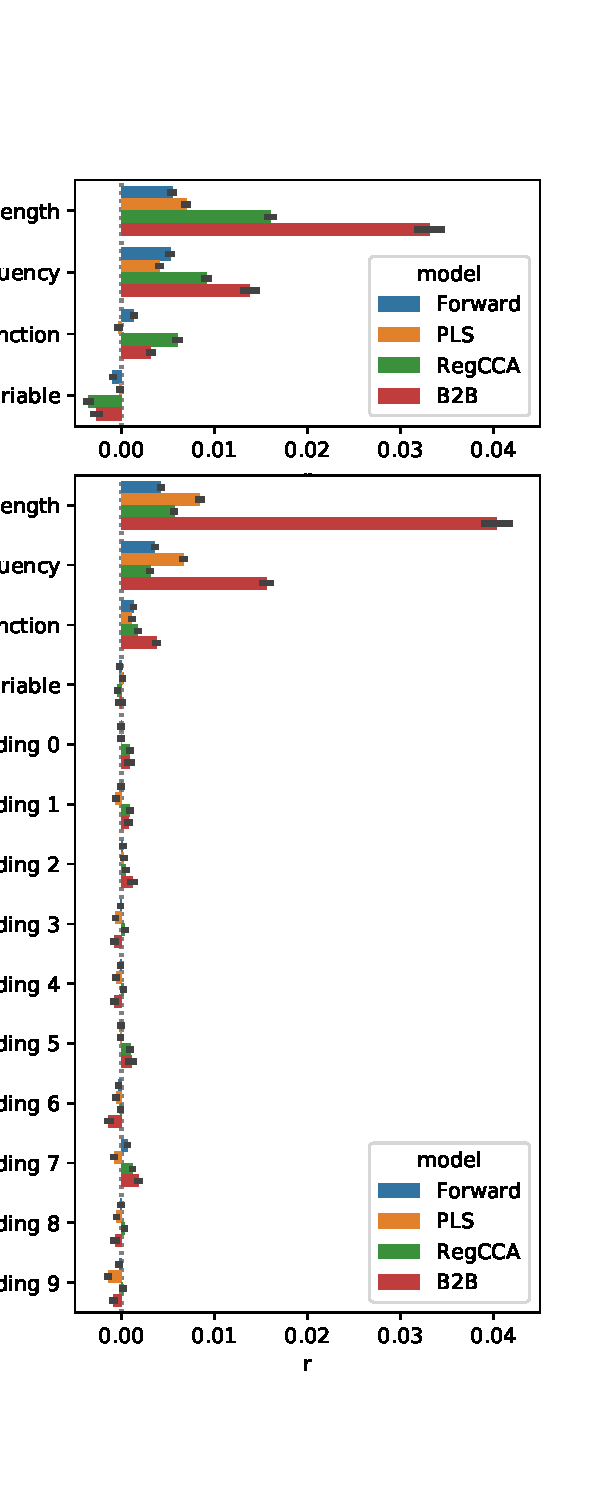
\includegraphics[width=0.5\linewidth]{figures/compare_embeddings.pdf}
  \caption{Comparison of $\Delta R$ when the models are tested on four variables (top) and when the models are tested on an these four variables as well as another 10 word-embedding features (bottom). These results illustrate that, unlike Regularized CCA, B2B remains robust even when the number of tested factors increases.
  \label{fig:embeddings}}
\end{figure}
